\documentclass[12pt, a4paper]{article}

\usepackage[a4paper, margin=2cm]{geometry}
\usepackage{setspace}
\usepackage[portuguese]{babel}
\usepackage{graphicx}

\chardef\_=`_

\title{\textbf{LI3 - Relatório da Fase I - Grupo 12}}
\author{
	Humberto Gomes (A104348) \\
	José Lopes     (A104541) \\
	José Matos     (A100612) \\
}
\date{novembro de 2023}

\begin{document}
\maketitle
\onehalfspacing
\setlength{\parskip}{\baselineskip}
\setlength{\parindent}{0pt}

\begin{abstract}
    Este relatório tem como intuito explicar a estrutura do nosso trabalho prático para a UC de LI3.
    Como o foco principal desta UC é a modularização e o encapsulamento do código, este documento
    descreve como tal for conseguido, justificando as nossas decisões a este nível. O objetivo do
    projeto para a 1.ª fase é o \emph{parsing} e validação de um \emph{dataset} contendo
    utilizadores, voos, passageiros em voos e reservas de hotéis, sobre o qual serão executadas
    \emph{queries}, das quais implementámos seis, fornecendo informação sobre a base de dados. O
    modo de organização e processamento destes dados também é descrito.
\end{abstract}

\section{Estrutura do trabalho}

Devido ao elevado número de módulos, um diagrama completo de módulos com relações de dependência
não cabe numa página A4, pelo que optámos por fazer vários diagramas, um para cada secção lógica
do programa. Mesmo assim, para reduzir a complexidade visual, não incluímos todas as relações de
dependência, mas apenas as mais relevantes.

A nossa convenção gráfica é a seguinte:

\begin{itemize}
	\item Um retângulo representa um módulo;
	\item Um retângulo com cantos arredondados representa uma estrutura de dados;
	\item $A \rightarrow B$ significa que o módulo $A$ depende do módulo $B$.
\end{itemize}

\subsection{Subsistema de \emph{parsing}}

\begin{center}
	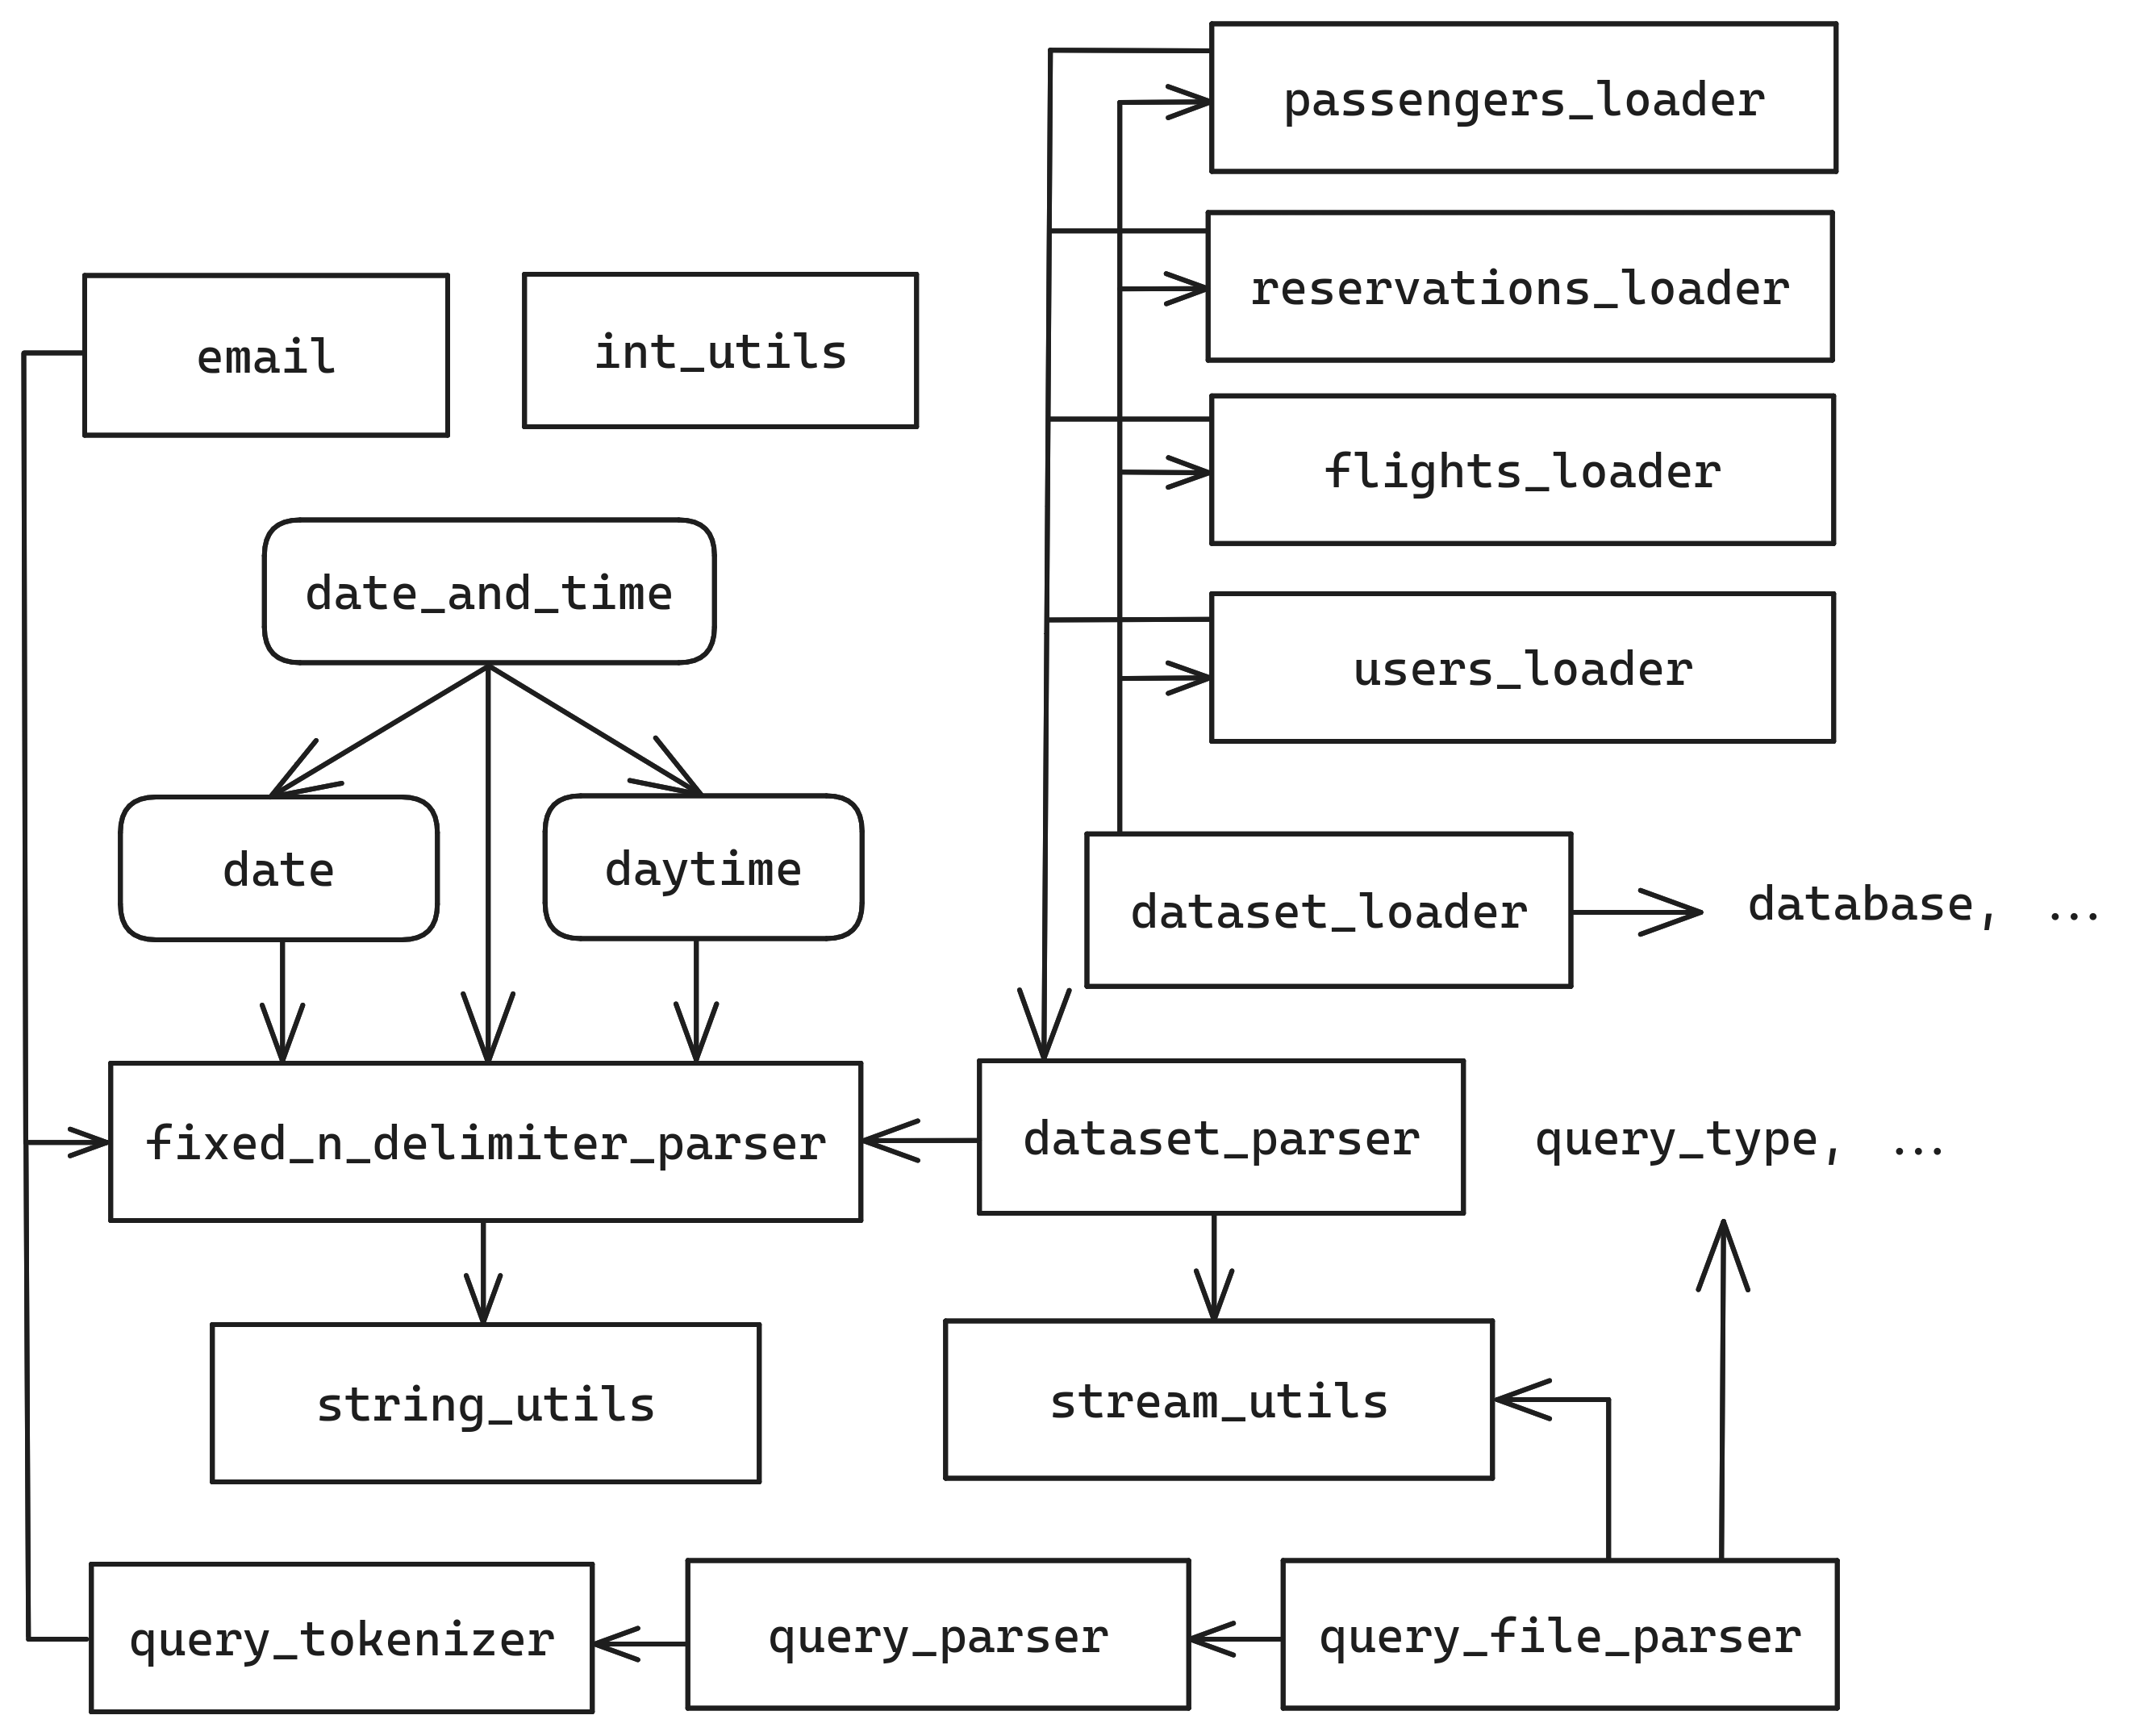
\includegraphics[scale=0.17]{res/parsing.png}
\end{center}

O nosso sistema de \emph{parsing} começa com \emph{tokenizadores}, que separam \emph{strings} e
ficheiros por um delimitador (\texttt{string\_utils} e \texttt{stream\_utils}, respetivamente).
Sobre estes é construído o caso mais específico do \texttt{fixed\_n\_delimiter\_parser}, que espera
um número pré-determinado de \emph{tokens}, chamando um \emph{callback} diferente para cada um (uma
gramática genérica, definível pelo programador, define estes \emph{callbacks}). Este \emph{parser}
é utilizado para o \emph{parsing} de datas (\texttt{date}), horas de um dia (\texttt{daytime}),
combinações de datas e horas (\texttt{date\_and\_time}), linhas de um \emph{dataset} e validação de
\emph{emails} (\texttt{email}).

Para a análise de um ficheiro de \emph{dataset}, o \texttt{dataset\_parser}, também programável com
uma gramática, é responsável por separar o ficheiro por linhas, excluir a primeira linha de cada
ficheiro (o \emph{header} da tabela CSV), e \emph{tokenizar} cada linha, chamando os
\emph{callbacks} adequados. O \texttt{dataset\_loader}, não propriamente encaixado neste secção de
\emph{parsing}, é responsável por abrir cada ficheiro do \emph{dataset}, interagir com os
\emph{parsers} adequados, adicionando elementos à base de dados e registando os erros por eles
reportados nos ficheiros \texttt{*\_errors.csv}.

O \emph{parsing} de \emph{queries} requer um \emph{tokenizador} separado para lidar com aspas
(\texttt{query\_tokenizer}), um \emph{parser} para determinar o tipo de \emph{query} e se os seus
argumentos são válidos (\texttt{query\_parser}), e um \emph{parser} de um ficheiro com várias
\emph{queries} em várias linhas (\texttt{query\_file\_parser}).

\section{Otimização do uso de memória}

Dado que os \emph{datasets} da 2.ª fase serão de maior dimensão, preocupámo-nos desde já com a
quantidade de memória utilizada, de modo não sermos futuramente obrigados a reescrever partes
significativas do nosso código.

\subsection{Observação do \emph{dataset} e das \emph{queries}}

Pudemos observar que alguns campos do \emph{dataset} nunca precisavam de estar presentes no
\emph{output} de nenhuma \emph{query} (ex: o \emph{email} de um utilizador), pelo que era escusado
o seu armazenamento na base de dados, sendo apenas necessária a sua validação durante o
\emph{parsing}. Ademais, por observação dos \emph{datasets} em si, pudemos concluir que é possível
armazenar certos campos como estruturas de dados mais compactas (ex: o identificador de um voo
pode ser armazenado como um inteiro, em vez de uma \emph{string}).

\subsection{Tipos opacos}

Um dos nossos obstáculos principais foi a forma como tipos opacos são implementados em C, que,
devido à sua natureza de apontador, exigem uma alocação por cada instanciamento. Esta secção
descreve como, mantendo o encapsulamento dos tipos, conseguimos definir tipos de dados opacos sem
estas limitações.

\subsubsection{Datas e horas}

De modo à \texttt{struct} de uma entidade (como um utilizador) poder conter, no seu interior, uma
data ou uma hora, sem alocações, estas são representadas como inteiros. Para modificar estes
inteiros, o módulo do tipo de dados usa uma \texttt{union}, como é visível abaixo no exemplo das
datas:


\begin{spacing}{1}
\begin{center}
    \begin{tabular}{ |l|l| }
        \hline
        \emph{include/utils/date.h}: & \emph{src/utils/date.c}: \\
		& \\
		\texttt{typedef int32\_t date\_t;} & \texttt{typedef union \{} \\
										   & \texttt{\hspace{0.5cm}date\_t date;} \\
                                           & \texttt{} \\
                                           & \texttt{\hspace{0.5cm}struct \{} \\
                                           & \texttt{\hspace{1cm}uint16\_t year;} \\
                                           & \texttt{\hspace{1cm}uint8\_t month, day;} \\
                                           & \texttt{\hspace{0.5cm}\} fields;} \\
                                           & \texttt{\} date\_union\_helper\_t;} \\
        \hline
    \end{tabular}
\end{center}
\end{spacing}

\subsubsection{Alocação de entidades em \emph{pools}}

Para evitar uma chamada de \texttt{malloc} por cada entidade no \emph{dataset}, procurámos alocar
grandes blocos contíguos de memória de uma vez (\emph{pools}), cada um contendo várias entidades.
No entanto, como o único aspeto de um tipo opaco exposto no \emph{header file} é um apontador, não
se sabe o tamanho da estrutura inerente a que o apontador se refere, impossibilitando a existência
destas \emph{pools}. Para endereçar este problema, adicionámos um método \texttt{\_sizeof} a cada
entidade que pretendíamos colocar em \emph{pools} (ex: \texttt{user\_sizeof}). A implementação
deste método, no ficheiro C, tem acesso à \texttt{struct} interna, podendo simplesmente ser
implementado como \texttt{return sizeof(user\_t);}.

\end{document}
